\section{Reconstruction}
\label{sec:Reconstruction}
The reconstruction process begins with either real or simulated data and proceeds to reconstruct progressively higher-level objects step-by-step, culminating in scifi tracks and trackpoints. The digits, real or simulated, are passed to the same set of MAUS modules and the reconstruction proceeds identically for either case from that point. The reconstruction process is illustrated in figure~\ref{fig:DataFlow} and is described in the sections that follow.

\begin{figure}[tb]
  \begin{center}
    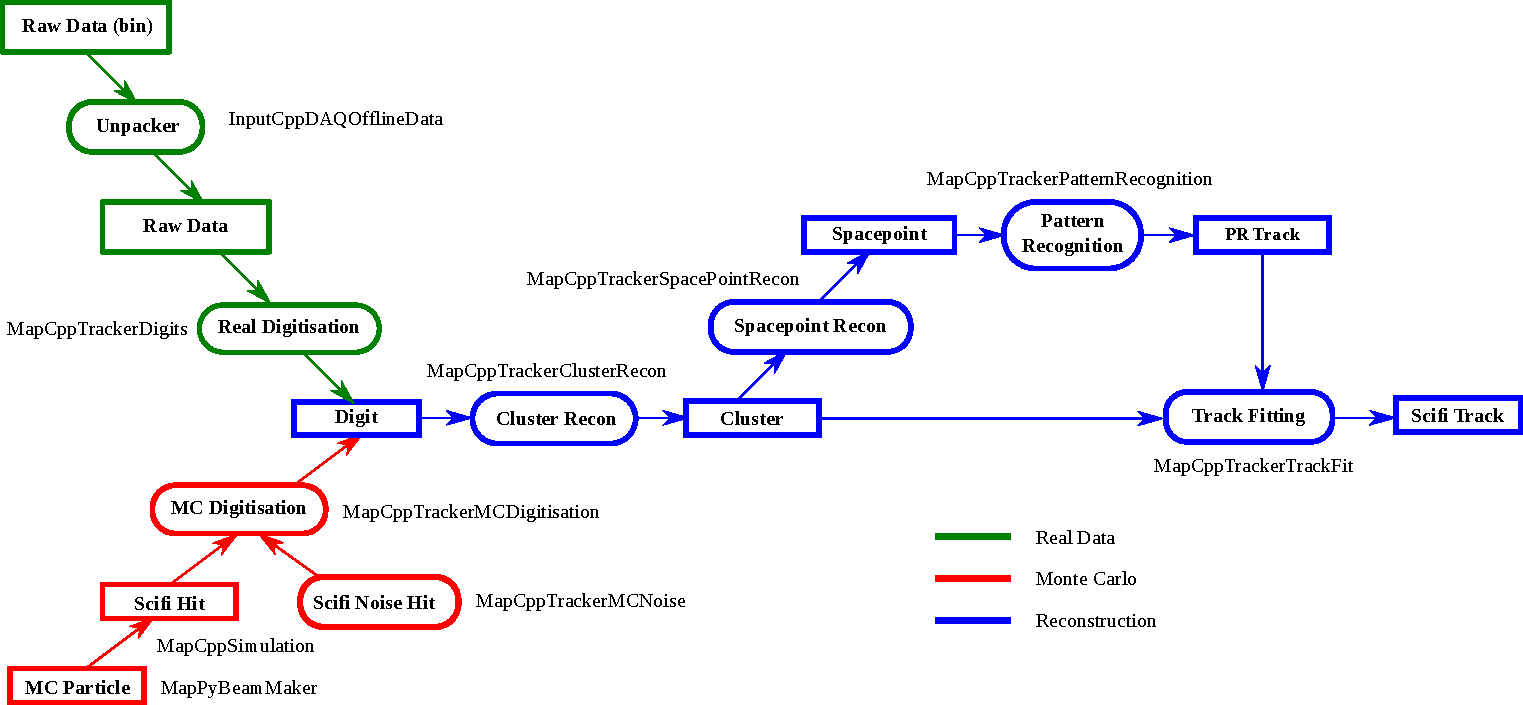
\includegraphics[width=0.95\linewidth]{07-Reconstruction/DataFlow2016.pdf}
    \caption{\label{fig:DataFlow} The reconstruction data flow. Data originates either from simulated or real-data, the two branches merge after digitisation, after which the reconstruction proceeds identically.  The relevant MAUS modules for each step are indicated.}
  \end{center}
\end{figure}

  \subsection{Digitization}
  \label{subsec:Digitization}
  For real-data the signal from the tracker ADCs is recorded by the DAQ system.  Channel-by-channel calibration constants are used to convert the ADC value to a signal in NPE and the DAQ channel number to tracker channel number.  This information is then used to form a digit.  The analogous process for Monte Carlo data is described in section~\ref{sec:Simulation}.

  \subsection{Cluster Reconstruction}
  \label{subsec:Clustering}
  The clustering algorithm loops over every combination of pairs of digits in a scifi event and combines any that occur in neighbouring channels. In the case of a multi-digit cluster, the unweighted average channel value is used to define the plane coordinate, $\alpha$, and the NPE is summed.

  \subsection{Spacepoint Reconstruction}
  \label{subsec:SpacepointReconstruction}
  For each station the constituent planes are searched for clusters that can be used to form a spacepoint. Spacepoints are constructed from clusters from all three planes (a triplet spacepoint) or for any two out of the three planes (a doublet spacepoint). 

  To determine which clusters from each plane originate from the same track, ``Kuno's conjecture''~\cite{MiceTrackers} is used: for a given triplet spacepoint the sum of the channel numbers of each cluster will be a constant.  So if $n^u$, $n^v$ and $n^w$ are the fibre numbers of the clusters in $u$, $v$ and $w$ and $n^u_0$, $n^v_0$ and $n^w_0$ are the corresponding central channel numbers. Three clusters form a space point if:
  \begin{equation}
    | (n^u + n^v + n^w) - (n^u_0 + n^v_0 + n^w_0) | < K \, .
  \end{equation}
  where $K$ is a constant, taken by default to be 3.0. The clusters are sorted according to NPE, with higher NPE clusters being matched using Kuno's conjecture first. 
  
  Once all triplet spacepoints have been found, doublet spacepoints are created from pairs of remaining clusters, the only selection criteria applied being that the crossing point of the two channels is within the tracker radius. 
  
  Spacepoint positioning is determined from the cluster measurements, $\alpha$ (see section~\ref{subsec:PlaneAndClusters}) and the known plane orientations for those measurements. All clusters selected as belonging to the same spacepoint must interesect. Using two clusters the second plane coordinate $\beta$ may be calculated using knowledge of the plane orientations. This then expresses the crossing point in the plane coordinate system, which can be simply rotated into the station $(x, y)$ coordinate system. In the case of a triplet spacepoint three crossing points are present, the average of which is used to define the final spacepoint position.

% For overlapping clusters:
%   
%     \begin{equation}
%     \begin{pmatrix}
%     \alpha_1 \\ \beta_1
%     \end{pmatrix} = R_{1}^{-1} R_2
%     \begin{pmatrix}
%     \alpha_2 \\ \beta_2
%     \end{pmatrix}
%     \end{equation}   
% \noindent

  % \subsubsection{Crossing Point Calculation}
  % \label{subsubsec:CrossingPointCalculation}

  \subsection{Pattern Recognition}
  \label{subsec:PatternRecognition}

  Pattern recognition is based on looping over different combinations of spacepoints and performing a fit using a linear-least-squares technique. There are separate algorithms for the straight-track (no field) case and the helical-track case.

   \subsubsection{Helical Pattern Recognition}
   \label{subsubsec:HelicalPatternRecognition}

   %The helical pattern recognition is performed in cylindrical co-ordinates $(r, \phi, z)$ where the turning angle $\phi$ defined for $0 \rightarrow \infty$ is distinguished from $\phi '$ the reduced turning angle defined for $0 \rightarrow 2\pi$. 
   
   The helical pattern recognition is performed in cylindrical co-ordinates $(r, \phi, z)$, where $r$ is the helix radius, $\phi$ the turning angle in the transverse plane, and $z$ is the longitudinal coordinate. An additional coordinate, $s$ the distance the particle travels in the transverse plane, is also defined. The helix is then parameterised by: the circle centre $x_c$, $y_c$ and the radius, $r$, in the transverse plane; $s_0$ the value of $s$ where the helix crosses the tracker reference plane; and $t_s = ds/dz$, which describes the tightness of the coiling. %$\phi_0$, the angle of the track as it crosses the tracker reference plane, equivalent to $s_0$, is also used. 

   To find a track one spacepoint is selected from each station and a circle is fitted in the $(r, \phi')$ projection. If the $\chi^2$ of this fit is sufficiently small (by default less than 15.0 multiplied by the number of degrees of freedom, NDF) then the value of $\phi$ is used to generate $s$ and a straight line fit is performed in the $(z,s)$ plane and, if the $\chi^2$ in this projection is also small (by default less than 4.0 multiplied by the NDF), the track is accepted as a track candidate. Once all the different possible combinations of spacepoints have been tried the track candidate with the lowest combined $\chi^2$ is accepted. Once every possible track with a spacepoint in all 5 stations has been found, the procedure is repeated looking for tracks with spacepoints in only 4 of the 5 stations. %$\phi$ itself is determined from $\phi'$ by exploiting the different distances in $z$ between successive tracker stations.  The change in $\phi$ between the hits in any two stations, divided by the distance between those stations, gives a constant which is the same for any pair of hits.  This can then be used to infer the true values of $\phi$.
   %TODO Define small
   
   %Tracks with momentum almost parallel to the solenoid axis (i.e. with low transverse momentum, $p_T$) will not suffer an appreciable bend and will not be found by the helix search and so any spacepoints remaining after the helical-tracks have been found are passed to the straight-track finding algorithm.

    \subsubsection{Straight Line Pattern Recognition}
    \label{subsubsec:StraightLinePatternRecognition}

    % Straight lines are fitted to the spacepoints when there is no magnetic field and on any spacepoints remaining after the helix fit is complete. The latter is to identify tracks with a small $p_T$ which are not bent sufficiently in the magnetic field to form a recognisable helix (it has been observed from Monte Carlo studies that the efficiency of the helix finding algorithm begins to tail off for tracks with $p_T < 10 MeV/c$).

    The straight-track finding is performed in Cartesian coordinates. The track parameters are $(x_0, y_0, t_x, t_y)$, where: $(x_0$, $y_0)$ is the position at which the track crosses the tracker reference surface; $t_x = dx/dz$; and $t_y = dy/dz$. Two spacepoints are chosen in the outer stations and a road is created between them. Any spacepoints in the road are fitted in the $(x,z)$ and $(y,z)$ planes. If the $\chi^2$ of the fits is small (by default less than 4.0 multiplied by the NDF) a candidate track is formed. Once all possible spacepoint combinations have been tried the track candidate with the lowest $\chi^2$ is selected. As in the helical case, following the completion of the full 5 point track search, tracks with spacepoints in 4 out of the 5 stations are searched for. For the straight case only, following the completion of the search for 4 point tracks, a search is also made for tracks with spacepoints in only 3 out of the 5 stations. 

   \subsection{Track Fit}
   \label{subsec:FinalTrackFit}
   The final track fit was implemented using a track-orientated Kalman filter~\cite{Fruhwirth,Billoir}, which can be shown to be an optimal linear fitter, that takes into account all correlations and measurements, for a linear system. The Kalman filter is an iterative algorithm that incrementally propagates an estimate of the current track state between measurement planes, using measurement information to ``filter'' the state, improving the estimate of the track state.
   
   For the helical-track fit, the system is only approximately linear, hence an extended Kalman filter~\cite{Goodwin} was implemented which analytically propagates the track states between measurements, while the covariance matrices are propagated using a first-order linear approximation to the non-linear system.

   Pattern recognition provides a set of clusters that are associated with a track, which passed the selection criteria, and a parameterisation of that track based on a least-squares fit to the points by a helix or a straight line as appropriate. The track parameters calculated from the least-squares fit are used to provide the seed for the Kalman fit and the cluster information is used as the measurement data. The flexibility of the Kalman algorithm permits the effects of individual planes (multiple Coulomb scattering, MCS, and energy loss) and the effect of the helium gas within the tracker to be accounted for between each measurement point.
%      \subsubsection{Kalman Filtering}
% 
%      The track is modelled as a discrete state-space function of $z$ (the direction of the beam), indicated by the subscript, $k$, where each tracker plane corresponds to a trackpoint and contains a measurement and a track state. Equation~\ref{equ:kalman_system_equation} describes how the true state-space vector, $\mathbf{x}_{k,t}$, is assumed to propagate to a subsequent measurement plane. The matrix, $\mathbf{F}_k$, is the Kalman Propagator and describes the first order description of the propagation between measurement planes. $\mathbf{w}_k$ represents some ``process noise'', which may affect the system between the two measurement planes and is assumed to be Gaussian distributed white noise.
%     \begin{equation}
%       \mathbf{x}_{k,t} = \mathbf{F}_{k-1}\mathbf{x}_{k-1,t} + \mathbf{w}_{k-1}
%       \label{equ:kalman_system_equation}
%     \end{equation}
%     \begin{equation*}
%       \textrm{exp}(\mathbf{w}) = 0 \quad\quad \textrm{and} \quad\quad \textrm{cov}(\mathbf{w}) = \mathbf{Q}
%     \end{equation*}
%      
%      The tracker measurements are interpreted in a different state-space to the track, allowing measurements of any dimension to be used to filter the track. Equation~\ref{equ:kalman_measurement_equation} describes how the true track state is ``measured'' to be transformed into the measurement space. The matrix, $\mathbf{H}_k$, is the Kalman Measurement Matrix and describes, to first order, the transformation from track state-space to the measurement state-space. $\mathbf{\varepsilon}_k$ represents some ``measurement noise'' which may smear the measurement of the true state-space, it is also assumed to be Gaussian distributed.
%     \begin{equation}
%       \mathbf{m}_k = \mathbf{H}_kx_{k,t} + \mathbf{\varepsilon}_k
%       \label{equ:kalman_measurement_equation}
%     \end{equation}
%     \begin{equation*}
%       \textrm{exp}(\mathbf{\varepsilon}) = 0 \quad\quad \textrm{and} \quad\quad \textrm{cov}(\mathbf{\varepsilon}) = \mathbf{V}
%     \end{equation*}
% 
%     For each measurement plane that contains a measurement, the current estimate for the track state vector is ``filtered'' using the measurement information. This is achieved using the residual between the estimate for the track state and the measurement data, in the measurement state-space. Equation~\ref{equ:kalman_state_filtered} describes how the predicted state vector, $\mathbf{x}_{k}^{k-1}$ is filtered using the Kalman Gain Matrix, $\mathbf{K}_k$, to produce the filtered track estimate, $\mathbf{x}_k$. Equation~\ref{equ:kalman_gain_matrix} defines the Kalman Gain Matrix.
%     \begin{equation}
%       \mathbf{x}_k = \mathbf{x}_k^{k-1} + \mathbf{K}_k ( \mathbf{m}_k - \mathbf{H}_k \mathbf{x}_k^{k-1} )
%       \label{equ:kalman_state_filtered}
%     \end{equation}
%     The predicted covariance matrix, $\mathbf{C}_k^{k-1}$, is filtered in a similar  fashion to produce the filtered covariance matrix, $\mathbf{C}_k^{k}$, as described in equation~\ref{equ:kalman_covariance_filtered}:
%     \begin{equation}
%       \mathbf{C}_k = ( \mathbf{I} - \mathbf{K}_k \mathbf{H}_k ) \mathbf{C}_k^{k-1}
%       \label{equ:kalman_covariance_filtered}
%     \end{equation}
%     The Kalman Gain matrix is calculated by:
%     \begin{equation}
%       \mathbf{K}_k = \mathbf{C}_k^{k-1} \mathbf{H}_k^\mathsf{T} (\mathbf{V}_k + \mathbf{H}_k \mathbf{C}_k^{k-1} \mathbf{H}_k^\mathsf{T})^{-1}
%       \label{equ:kalman_gain_matrix}
%     \end{equation}
% 
%     The sequence of prediction and filtering is repeated for all the measurement planes, starting from station~5, plane~2, where the predicted state vector and covariance matrix is determined from the pattern recognition fit parameters, to station~1, plane~0, the reference plane. Once the reference plane has been reached, the state vector will have been sequentially filtered using all the measurements in turn to create the optimal estimate of the track state at that plane. The fit can then be smoothed, whereby the optimal state vector is propagated in reverse down the length of the track, such that all the subsequent measurements can be used to re-adjust previous state vector estimates. This is described in~\cite{Fruhwirth}


%     \subsubsection{The MAUS Kalman Filter Implementation}
    The Kalman filter was written from scratch. In order to make the implementation flexible and re-usable the core algorithm was implemented without any dependencies on phase-space dimensions or physical effects. % Due to this only the system specific functionality need be provided for a complete implementation.
    The principal components of the implementation are: propagation routines for both helical and straight-tracks; a measurement routine that transforms the track state-space into the measurement state-space; and approximations for the process and measurement noise.
    
    The measurements correspond to individual clusters, hence the parameter $\alpha$ (see section~\ref{subsec:PlaneAndClusters}) forms a one-dimensional measurement state. The measurement noise corresponds to the statistical spread of measurements within a single channel of width $w$ in the tracker readout. If the channel is modelled as a top-hat function, the variance of the function is $w^2/12$. Therefore the measurement noise was taken to be $w/\sqrt{12}$ for all clusters.

    The process noise was implemented as a combination of MCS and energy straggling. The energy loss is calculated using the Bethe formula~\cite{PDG}, for the most probable energy loss, and applied during the propagation stage. The noise term itself is calculated per increment as an RMS scattering angle using an implementation of the Highland formula~\cite{Highland}, in a fashion almost identical to the GEANT4 implementation:
    \begin{equation}
      \theta_{RMS} = \frac{13.6\textrm{MeV/c}}{\beta c p} Z \frac{x}{X_0}\left( 1 + 0.038 \ln\left(\frac{x}{X_0} \right)\right)
      \label{equ:highland_formula}
    \end{equation}
    where $\theta_{RMS}$ is the RMS scattering angle through a finite length of material, $\beta c$, $p$ and $Z$ are the velocity, momentum and charge of the particle in question, $x$ is the distance travelled and $X_0$ the radiation length of the material. Although the RMS scattering angle does not form a Gaussian distribution, the first order approximation is believed to be sufficient.

    In contrast to pattern recognition, the Kalman filter uses a different state-space model, ($x$, $p_x$, $y$, $p_y$, $q/p_z$) rather than ($x_c$, $y_c$, $r$, $s_0$, $t_s$). This permits energy loss and multiple Coulomb scattering to be modelled linearly and implmentated using a more simple set of algorithms. 
    
    % The longitudinal components, however, are less easily modelled due to small angle scattering, such that the reconstruction of $p_z$ from the final track fit is sensitive to the accuracy of the pattern recognition stage.

%    \subsubsection{Goodness of fit}
%    For each fitted track, a test statistic is computed, which is the $\chi^2$ sum over all the trackpoints. It is calculated by $\chi^2\sum_{k=0}^{k=n}\chi_k^2$ where each chisquared update is given by $\chi_{k}^{2}=\mathbf{r}_{k}^{T}\mathrm{R}_{k}^{-1}\mathbf{r}_{k}$: where $r_{k}$ is the residual computed from the filtered state vector. $r_{k}=\mathbf{m}_{k}-\mathrm{H}_{k}\mathbf{a}_{k}$: where $\mathbf{m}_{k}$ is the $k^{th}$  measured point; $\mathbf{a}_{k}$ is the best Kalman estimate of track state vector at the $k^{th}$ intersection point and $\mathrm{H}_{k}$ is the matrix which projects the state vector of the track into the measurement space. $\mathrm{R}_{k}$ is the covariance matrix of the residuals and is given by  $\mathrm{R}_{k}=\mathrm{V}_{k}-\mathrm{H}_{k}\mathrm{C}_{k}\mathrm{H}_{k}^{T}$ where $\mathrm{V}_{k}$ is the measurement covariance matrix and $\mathrm{C}_{k}$ is the projected variance matrix. This definition of  $\chi^{2}$  takes into account correlations in the measurement predictions and, combined with the number of degrees of freedom of the track fit, is used to generate a {\it p-value} for the track, which we use as a measure of fit quality.


%\begin{equation}
%\chi_{k}^{2}=\mathbf{r}_{k}^{T}\mathrm{R}_{k}^{-1}\mathbf{r}_{k}.
%\end{equation}





  
